\documentclass[tikz,border=4pt]{standalone}
\usepackage{amsmath,amssymb}
\usetikzlibrary{arrows.meta}
% Grupo Nostradamus - lenguaje visual TikZ
\definecolor{nostranavy}{HTML}{061426}
\definecolor{nostrateal}{HTML}{078C95}
\definecolor{nostracyan}{HTML}{65DCE5}
\definecolor{nostragold}{HTML}{F5C542}
\newcommand{\sen}{\operatorname{sen}}

\begin{document}
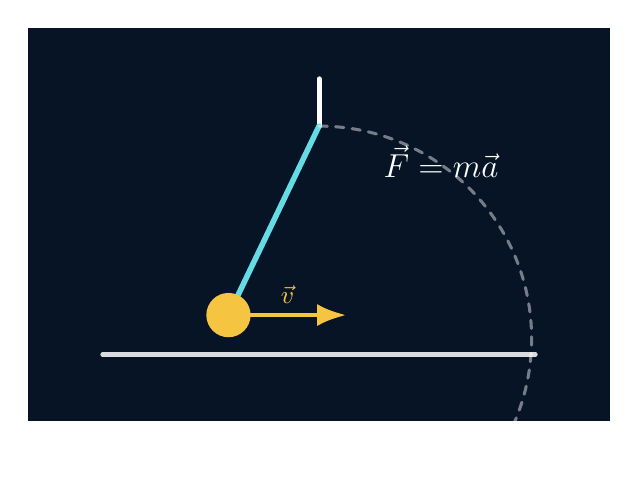
\begin{tikzpicture}[line cap=round,line join=round,>=Latex]
\fill[nostranavy] (-3.7,-2.5) rectangle (3.7,2.5);
\draw[white,line width=1.8pt] (0,1.85)--(0,1.25);
\draw[nostracyan,line width=2pt] (0,1.25)--(-1.15,-1.15);
\fill[nostragold] (-1.15,-1.15) circle (8pt);
\draw[white,opacity=.45,line width=1.1pt,dashed] (0,1.25) arc[start angle=90,end angle=-35,radius=2.7];
\draw[white,opacity=.85,line width=1.5pt] (-2.75,-1.65)--(2.75,-1.65);
\draw[nostragold,->,line width=1.7pt] (-1.15,-1.15)--(.35,-1.15) node[midway,above,font=\bfseries\small] {$\vec v$};
\node[white,font=\bfseries\large] at (1.55,.80) {$\vec F=m\vec a$};
\end{tikzpicture}
\end{document}
